\fancyhead[LE]{\fontsize{8.5pt}{10pt}\selectfont\textbf{\textsf{\thepage}}\quad \textbf{\textsf{CHƯƠNG 1}}\quad \textsf{Các hàm số và Mô hình}}
\fancyhead[RO]{\fontsize{8.5pt}{10pt}\selectfont\textsf{MỤC 1.1}\quad \textbf{\textsf{\thepage}}}

\noindent
\begin{minipage}[t]{0.265\textwidth}
    \fontsize{8pt}{10pt}\selectfont
    \vspace{3pt}
    \centering
    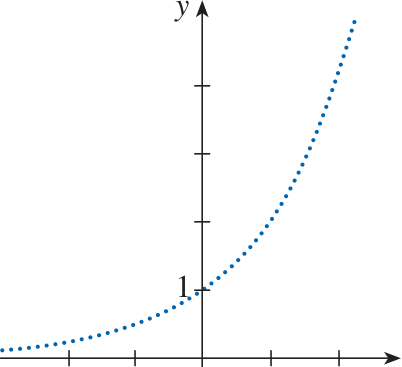
\includegraphics[width=0.82\linewidth]{images/p0081_fig1.png}\\[4pt]
    \parbox{0.92\linewidth}{\raggedright \textbf{\textsf{HÌNH 1}}\\Biểu diễn của $y = 2^x$, $x$ hữu tỉ}\par

    \vspace{3pt}
    \parbox{0.92\linewidth}{\raggedright Chứng minh cho khẳng định này được trình bày trong J. Marsden và A. Weinstein, \textit{Calculus Unlimited} (Menlo Park, CA: Benjamin/Cummings, 1981).}\par

    \vspace{3pt}
    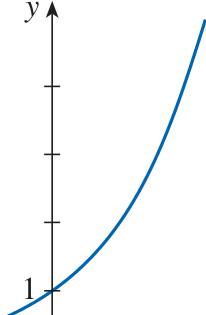
\includegraphics[width=0.82\linewidth]{images/p0081_fig2.png}\\[4pt]
    \parbox{0.92\linewidth}{\raggedright \textbf{\textsf{HÌNH 2}}\\$y = 2^x$, $x$ thực}\par
\end{minipage}%
\hfill
\begin{minipage}[t]{0.708\textwidth}
    \fontsize{8.8pt}{11.5pt}\selectfont
    Nếu $x = 0$, thì $b^0 = 1$, và nếu $x = -n$, trong đó $n$ là một số nguyên dương, thì
    \[
    b^{-n} = \frac{1}{b^n}
    \]
    Nếu $x$ là một số hữu tỉ, $x = p/q$, trong đó $p$ và $q$ là các số nguyên và $q > 0$, thì
    \[
    b^x = b^{p/q} = \sqrt[q]{b^p} = (\sqrt[q]{b})^p
    \]
    Nhưng ý nghĩa của $b^x$ là gì nếu $x$ là một số vô tỉ? Chẳng hạn, $2^{\sqrt{3}}$ hay $5^\pi$ có nghĩa là gì?

    Để giúp trả lời câu hỏi này, trước tiên ta quan sát đồ thị của hàm số $y = 2^x$, với $x$ là số hữu tỉ. Một hình ảnh minh họa cho đồ thị này được thể hiện trong Hình~1. Chúng ta muốn mở rộng miền xác định của $y = 2^x$ để bao gồm cả các số hữu tỉ và vô tỉ.

    Có những ``lỗ thủng'' trên đồ thị ở Hình~1 tương ứng với các giá trị vô tỉ của $x$. Ta muốn lấp đầy các lỗ thủng này bằng cách định nghĩa $f(x) = 2^x$, với $x \in \mathbb{R}$, sao cho $f$ là một hàm đồng biến. Cụ thể, vì số vô tỉ $\sqrt{3}$ thỏa mãn
    \[
    1.7 < \sqrt{3} < 1.8
    \]
    nên ta phải có
    \[
    2^{1.7} < 2^{\sqrt{3}} < 2^{1.8}
    \]
    và ta đã biết $2^{1.7}$ cùng với $2^{1.8}$ có nghĩa là gì vì $1.7$ và $1.8$ là các số hữu tỉ. Tương tự, nếu sử dụng các giá trị xấp xỉ tốt hơn cho $\sqrt{3}$, ta sẽ nhận được các xấp xỉ tốt hơn cho $2^{\sqrt{3}}$:
    \[
    \begin{alignedat}{2}
    1.73 &< \sqrt{3} < 1.74 &\quad \Rightarrow \quad 2^{1.73} &< 2^{\sqrt{3}} < 2^{1.74} \\
    1.732 &< \sqrt{3} < 1.733 &\quad \Rightarrow \quad 2^{1.732} &< 2^{\sqrt{3}} < 2^{1.733} \\
    1.7320 &< \sqrt{3} < 1.7321 &\quad \Rightarrow \quad 2^{1.7320} &< 2^{\sqrt{3}} < 2^{1.7321} \\
    1.73205 &< \sqrt{3} < 1.73206 &\quad \Rightarrow \quad 2^{1.73205} &< 2^{\sqrt{3}} < 2^{1.73206} \\
    &\;\;\vdots \qquad\qquad \vdots &&\;\;\vdots \qquad\qquad \vdots
    \end{alignedat}
    \]
    Có thể chứng minh được rằng có duy nhất một số lớn hơn tất cả các số
    \[
    2^{1.7},\quad 2^{1.73},\quad 2^{1.732},\quad 2^{1.7320},\quad 2^{1.73205},\quad \dots
    \]
    và nhỏ hơn tất cả các số
    \[
    2^{1.8},\quad 2^{1.74},\quad 2^{1.733},\quad 2^{1.7321},\quad 2^{1.73206},\quad \dots
    \]
    Ta định nghĩa $2^{\sqrt{3}}$ chính là số này. Bằng việc sử dụng quá trình xấp xỉ nêu trên, ta có thể tính được giá trị của nó chính xác đến sáu chữ số thập phân:
    \[
    2^{\sqrt{3}} \approx 3.321997
    \]
    Tương tự, ta có thể định nghĩa $2^x$ (hoặc $b^x$, nếu $b > 0$) với $x$ là bất kỳ số vô tỉ nào. Hình~2 cho thấy cách mà tất cả các lỗ thủng trong Hình~1 đã được lấp đầy để tạo thành đồ thị hoàn chỉnh của hàm số $f(x) = 2^x$, $x \in \mathbb{R}$.
\end{minipage}